
%% bare_conf.tex
%% V1.4b
%% 2015/08/26
%% by Michael Shell
%% See:
%% http://www.michaelshell.org/
%% for current contact information.
%%
%% This is a skeleton file demonstrating the use of IEEEtran.cls
%% (requires IEEEtran.cls version 1.8b or later) with an IEEE
%% conference paper.
%%
%% Support sites:
%% http://www.michaelshell.org/tex/ieeetran/
%% http://www.ctan.org/pkg/ieeetran
%% and
%% http://www.ieee.org/

%%*************************************************************************
%% Legal Notice:
%% This code is offered as-is without any warranty either expressed or
%% implied; without even the implied warranty of MERCHANTABILITY or
%% FITNESS FOR A PARTICULAR PURPOSE! 
%% User assumes all risk.
%% In no event shall the IEEE or any contributor to this code be liable for
%% any damages or losses, including, but not limited to, incidental,
%% consequential, or any other damages, resulting from the use or misuse
%% of any information contained here.
%%
%% All comments are the opinions of their respective authors and are not
%% necessarily endorsed by the IEEE.
%%
%% This work is distributed under the LaTeX Project Public License (LPPL)
%% ( http://www.latex-project.org/ ) version 1.3, and may be freely used,
%% distributed and modified. A copy of the LPPL, version 1.3, is included
%% in the base LaTeX documentation of all distributions of LaTeX released
%% 2003/12/01 or later.
%% Retain all contribution notices and credits.
%% ** Modified files should be clearly indicated as such, including  **
%% ** renaming them and changing author support contact information. **
%%*************************************************************************


% *** Authors should verify (and, if needed, correct) their LaTeX system  ***
% *** with the testflow diagnostic prior to trusting their LaTeX platform ***
% *** with production work. The IEEE's font choices and paper sizes can   ***
% *** trigger bugs that do not appear when using other class files.       ***                          ***
% The testflow support page is at:
% http://www.michaelshell.org/tex/testflow/



\documentclass[conference]{IEEEtran}
% Some Computer Society conferences also require the compsoc mode option,
% but others use the standard conference format.
%
% If IEEEtran.cls has not been installed into the LaTeX system files,
% manually specify the path to it like:
% \documentclass[conference]{../sty/IEEEtran}





% Some very useful LaTeX packages include:
% (uncomment the ones you want to load)


% *** MISC UTILITY PACKAGES ***
%
%\usepackage{ifpdf}
% Heiko Oberdiek's ifpdf.sty is very useful if you need conditional
% compilation based on whether the output is pdf or dvi.
% usage:
% \ifpdf
%   % pdf code
% \else
%   % dvi code
% \fi
% The latest version of ifpdf.sty can be obtained from:
% http://www.ctan.org/pkg/ifpdf
% Also, note that IEEEtran.cls V1.7 and later provides a builtin
% \ifCLASSINFOpdf conditional that works the same way.
% When switching from latex to pdflatex and vice-versa, the compiler may
% have to be run twice to clear warning/error messages.






% *** CITATION PACKAGES ***
%
%\usepackage{cite}
% cite.sty was written by Donald Arseneau
% V1.6 and later of IEEEtran pre-defines the format of the cite.sty package
% \cite{} output to follow that of the IEEE. Loading the cite package will
% result in citation numbers being automatically sorted and properly
% "compressed/ranged". e.g., [1], [9], [2], [7], [5], [6] without using
% cite.sty will become [1], [2], [5]--[7], [9] using cite.sty. cite.sty's
% \cite will automatically add leading space, if needed. Use cite.sty's
% noadjust option (cite.sty V3.8 and later) if you want to turn this off
% such as if a citation ever needs to be enclosed in parenthesis.
% cite.sty is already installed on most LaTeX systems. Be sure and use
% version 5.0 (2009-03-20) and later if using hyperref.sty.
% The latest version can be obtained at:
% http://www.ctan.org/pkg/cite
% The documentation is contained in the cite.sty file itself.






% *** GRAPHICS RELATED PACKAGES ***
%
\ifCLASSINFOpdf
   \usepackage[pdftex]{graphicx}
  % declare the path(s) where your graphic files are
  % \graphicspath{{../pdf/}{../jpeg/}}
  % and their extensions so you won't have to specify these with
  % every instance of \includegraphics
  % \DeclareGraphicsExtensions{.pdf,.jpeg,.png}
\else
  % or other class option (dvipsone, dvipdf, if not using dvips). graphicx
  % will default to the driver specified in the system graphics.cfg if no
  % driver is specified.
  % \usepackage[dvips]{graphicx}
  % declare the path(s) where your graphic files are
  % \graphicspath{{../eps/}}
  % and their extensions so you won't have to specify these with
  % every instance of \includegraphics
  % \DeclareGraphicsExtensions{.eps}
\fi
% graphicx was written by David Carlisle and Sebastian Rahtz. It is
% required if you want graphics, photos, etc. graphicx.sty is already
% installed on most LaTeX systems. The latest version and documentation
% can be obtained at: 
% http://www.ctan.org/pkg/graphicx
% Another good source of documentation is "Using Imported Graphics in
% LaTeX2e" by Keith Reckdahl which can be found at:
% http://www.ctan.org/pkg/epslatex
%
% latex, and pdflatex in dvi mode, support graphics in encapsulated
% postscript (.eps) format. pdflatex in pdf mode supports graphics
% in .pdf, .jpeg, .png and .mps (metapost) formats. Users should ensure
% that all non-photo figures use a vector format (.eps, .pdf, .mps) and
% not a bitmapped formats (.jpeg, .png). The IEEE frowns on bitmapped formats
% which can result in "jaggedy"/blurry rendering of lines and letters as
% well as large increases in file sizes.
%
% You can find documentation about the pdfTeX application at:
% http://www.tug.org/applications/pdftex





% *** MATH PACKAGES ***
%
%\usepackage{amsmath}
% A popular package from the American Mathematical Society that provides
% many useful and powerful commands for dealing with mathematics.
%
% Note that the amsmath package sets \interdisplaylinepenalty to 10000
% thus preventing page breaks from occurring within multiline equations. Use:
%\interdisplaylinepenalty=2500
% after loading amsmath to restore such page breaks as IEEEtran.cls normally
% does. amsmath.sty is already installed on most LaTeX systems. The latest
% version and documentation can be obtained at:
% http://www.ctan.org/pkg/amsmath





% *** SPECIALIZED LIST PACKAGES ***
%
%\usepackage{algorithmic}
% algorithmic.sty was written by Peter Williams and Rogerio Brito.
% This package provides an algorithmic environment fo describing algorithms.
% You can use the algorithmic environment in-text or within a figure
% environment to provide for a floating algorithm. Do NOT use the algorithm
% floating environment provided by algorithm.sty (by the same authors) or
% algorithm2e.sty (by Christophe Fiorio) as the IEEE does not use dedicated
% algorithm float types and packages that provide these will not provide
% correct IEEE style captions. The latest version and documentation of
% algorithmic.sty can be obtained at:
% http://www.ctan.org/pkg/algorithms
% Also of interest may be the (relatively newer and more customizable)
% algorithmicx.sty package by Szasz Janos:
% http://www.ctan.org/pkg/algorithmicx




% *** ALIGNMENT PACKAGES ***
%
%\usepackage{array}
% Frank Mittelbach's and David Carlisle's array.sty patches and improves
% the standard LaTeX2e array and tabular environments to provide better
% appearance and additional user controls. As the default LaTeX2e table
% generation code is lacking to the point of almost being broken with
% respect to the quality of the end results, all users are strongly
% advised to use an enhanced (at the very least that provided by array.sty)
% set of table tools. array.sty is already installed on most systems. The
% latest version and documentation can be obtained at:
% http://www.ctan.org/pkg/array


% IEEEtran contains the IEEEeqnarray family of commands that can be used to
% generate multiline equations as well as matrices, tables, etc., of high
% quality.




% *** SUBFIGURE PACKAGES ***
%\ifCLASSOPTIONcompsoc
%  \usepackage[caption=false,font=normalsize,labelfont=sf,textfont=sf]{subfig}
%\else
  \usepackage[caption=false,font=footnotesize]{subfig}
%\fi
% subfig.sty, written by Steven Douglas Cochran, is the modern replacement
% for subfigure.sty, the latter of which is no longer maintained and is
% incompatible with some LaTeX packages including fixltx2e. However,
% subfig.sty requires and automatically loads Axel Sommerfeldt's caption.sty
% which will override IEEEtran.cls' handling of captions and this will result
% in non-IEEE style figure/table captions. To prevent this problem, be sure
% and invoke subfig.sty's "caption=false" package option (available since
% subfig.sty version 1.3, 2005/06/28) as this is will preserve IEEEtran.cls
% handling of captions.
% Note that the Computer Society format requires a larger sans serif font
% than the serif footnote size font used in traditional IEEE formatting
% and thus the need to invoke different subfig.sty package options depending
% on whether compsoc mode has been enabled.
%
% The latest version and documentation of subfig.sty can be obtained at:
% http://www.ctan.org/pkg/subfig




% *** FLOAT PACKAGES ***
%
%\usepackage{fixltx2e}
% fixltx2e, the successor to the earlier fix2col.sty, was written by
% Frank Mittelbach and David Carlisle. This package corrects a few problems
% in the LaTeX2e kernel, the most notable of which is that in current
% LaTeX2e releases, the ordering of single and double column floats is not
% guaranteed to be preserved. Thus, an unpatched LaTeX2e can allow a
% single column figure to be placed prior to an earlier double column
% figure.
% Be aware that LaTeX2e kernels dated 2015 and later have fixltx2e.sty's
% corrections already built into the system in which case a warning will
% be issued if an attempt is made to load fixltx2e.sty as it is no longer
% needed.
% The latest version and documentation can be found at:
% http://www.ctan.org/pkg/fixltx2e


%\usepackage{stfloats}
% stfloats.sty was written by Sigitas Tolusis. This package gives LaTeX2e
% the ability to do double column floats at the bottom of the page as well
% as the top. (e.g., "\begin{figure*}[!b]" is not normally possible in
% LaTeX2e). It also provides a command:
%\fnbelowfloat
% to enable the placement of footnotes below bottom floats (the standard
% LaTeX2e kernel puts them above bottom floats). This is an invasive package
% which rewrites many portions of the LaTeX2e float routines. It may not work
% with other packages that modify the LaTeX2e float routines. The latest
% version and documentation can be obtained at:
% http://www.ctan.org/pkg/stfloats
% Do not use the stfloats baselinefloat ability as the IEEE does not allow
% \baselineskip to stretch. Authors submitting work to the IEEE should note
% that the IEEE rarely uses double column equations and that authors should try
% to avoid such use. Do not be tempted to use the cuted.sty or midfloat.sty
% packages (also by Sigitas Tolusis) as the IEEE does not format its papers in
% such ways.
% Do not attempt to use stfloats with fixltx2e as they are incompatible.
% Instead, use Morten Hogholm'a dblfloatfix which combines the features
% of both fixltx2e and stfloats:
%
% \usepackage{dblfloatfix}
% The latest version can be found at:
% http://www.ctan.org/pkg/dblfloatfix




% *** PDF, URL AND HYPERLINK PACKAGES ***
%
%\usepackage{url}
% url.sty was written by Donald Arseneau. It provides better support for
% handling and breaking URLs. url.sty is already installed on most LaTeX
% systems. The latest version and documentation can be obtained at:
% http://www.ctan.org/pkg/url
% Basically, \url{my_url_here}.




% *** Do not adjust lengths that control margins, column widths, etc. ***
% *** Do not use packages that alter fonts (such as pslatex).         ***
% There should be no need to do such things with IEEEtran.cls V1.6 and later.
% (Unless specifically asked to do so by the journal or conference you plan
% to submit to, of course. )


% correct bad hyphenation here
\hyphenation{op-tical net-works semi-conduc-tor}


\begin{document}
%
% paper title
% Titles are generally capitalized except for words such as a, an, and, as,
% at, but, by, for, in, nor, of, on, or, the, to and up, which are usually
% not capitalized unless they are the first or last word of the title.
% Linebreaks \\ can be used within to get better formatting as desired.
% Do not put math or special symbols in the title.
\title{NYC Green Taxis with Neural Network}


% author names and affiliations
% use a multiple column layout for up to three different
% affiliations
\author{\IEEEauthorblockN{Brittany Nicholls}
\IEEEauthorblockA{Department of Computer Science\\ and Electrical Engineering\\
University of Maryland, Baltimore County\\
Baltimore, Maryland 21250\\
Email: brn1@umbc.edu}}

% conference papers do not typically use \thanks and this command
% is locked out in conference mode. If really needed, such as for
% the acknowledgment of grants, issue a \IEEEoverridecommandlockouts
% after \documentclass

% for over three affiliations, or if they all won't fit within the width
% of the page, use this alternative format:
% 
%\author{\IEEEauthorblockN{Michael Shell\IEEEauthorrefmark{1},
%Homer Simpson\IEEEauthorrefmark{2},
%James Kirk\IEEEauthorrefmark{3}, 
%Montgomery Scott\IEEEauthorrefmark{3} and
%Eldon Tyrell\IEEEauthorrefmark{4}}
%\IEEEauthorblockA{\IEEEauthorrefmark{1}School of Electrical and Computer Engineering\\
%Georgia Institute of Technology,
%Atlanta, Georgia 30332--0250\\ Email: see http://www.michaelshell.org/contact.html}
%\IEEEauthorblockA{\IEEEauthorrefmark{2}Twentieth Century Fox, Springfield, USA\\
%Email: homer@thesimpsons.com}
%\IEEEauthorblockA{\IEEEauthorrefmark{3}Starfleet Academy, San Francisco, California 96678-2391\\
%Telephone: (800) 555--1212, Fax: (888) 555--1212}
%\IEEEauthorblockA{\IEEEauthorrefmark{4}Tyrell Inc., 123 Replicant Street, Los Angeles, California 90210--4321}}




% use for special paper notices
%\IEEEspecialpapernotice{(Invited Paper)}




% make the title area
\maketitle

% As a general rule, do not put math, special symbols or citations
% in the abstract
\begin{abstract}
NYC Green TAxi.  Use Neural Net.  Kaggle Competition. RMSE vs RMSLE
\end{abstract}

% no keywords




% For peer review papers, you can put extra information on the cover
% page as needed:
% \ifCLASSOPTIONpeerreview
% \begin{center} \bfseries EDICS Category: 3-BBND \end{center}
% \fi
%
% For peerreview papers, this IEEEtran command inserts a page break and
% creates the second title. It will be ignored for other modes.
\IEEEpeerreviewmaketitle




% An example of a floating figure using the graphicx package.
% Note that \label must occur AFTER (or within) \caption.
% For figures, \caption should occur after the \includegraphics.
% Note that IEEEtran v1.7 and later has special internal code that
% is designed to preserve the operation of \label within \caption
% even when the captionsoff option is in effect. However, because
% of issues like this, it may be the safest practice to put all your
% \label just after \caption rather than within \caption{}.
%
% Reminder: the "draftcls" or "draftclsnofoot", not "draft", class
% option should be used if it is desired that the figures are to be
% displayed while in draft mode.
%
%\begin{figure}[!t]
%\centering
%\includegraphics[width=2.5in]{myfigure}
% where an .eps filename suffix will be assumed under latex, 
% and a .pdf suffix will be assumed for pdflatex; or what has been declared
% via \DeclareGraphicsExtensions.
%\caption{Simulation results for the network.}
%\label{fig_sim}
%\end{figure}

% Note that the IEEE typically puts floats only at the top, even when this
% results in a large percentage of a column being occupied by floats.


% An example of a double column floating figure using two subfigures.
% (The subfig.sty package must be loaded for this to work.)
% The subfigure \label commands are set within each subfloat command,
% and the \label for the overall figure must come after \caption.
% \hfil is used as a separator to get equal spacing.
% Watch out that the combined width of all the subfigures on a 
% line do not exceed the text width or a line break will occur.
%
%\begin{figure*}[!t]
%\centering
%\subfloat[Case I]{\includegraphics[width=2.5in]{box}%
%\label{fig_first_case}}
%\hfil
%\subfloat[Case II]{\includegraphics[width=2.5in]{box}%
%\label{fig_second_case}}
%\caption{Simulation results for the network.}
%\label{fig_sim}
%\end{figure*}
%
% Note that often IEEE papers with subfigures do not employ subfigure
% captions (using the optional argument to \subfloat[]), but instead will
% reference/describe all of them (a), (b), etc., within the main caption.
% Be aware that for subfig.sty to generate the (a), (b), etc., subfigure
% labels, the optional argument to \subfloat must be present. If a
% subcaption is not desired, just leave its contents blank,
% e.g., \subfloat[].


% An example of a floating table. Note that, for IEEE style tables, the
% \caption command should come BEFORE the table and, given that table
% captions serve much like titles, are usually capitalized except for words
% such as a, an, and, as, at, but, by, for, in, nor, of, on, or, the, to
% and up, which are usually not capitalized unless they are the first or
% last word of the caption. Table text will default to \footnotesize as
% the IEEE normally uses this smaller font for tables.
% The \label must come after \caption as always.
%
%\begin{table}[!t]
%% increase table row spacing, adjust to taste
%\renewcommand{\arraystretch}{1.3}
% if using array.sty, it might be a good idea to tweak the value of
% \extrarowheight as needed to properly center the text within the cells
%\caption{An Example of a Table}
%\label{table_example}
%\centering
%% Some packages, such as MDW tools, offer better commands for making tables
%% than the plain LaTeX2e tabular which is used here.
%\begin{tabular}{|c||c|}
%\hline
%One & Two\\
%\hline
%Three & Four\\
%\hline
%\end{tabular}
%\end{table}


% Note that the IEEE does not put floats in the very first column
% - or typically anywhere on the first page for that matter. Also,
% in-text middle ("here") positioning is typically not used, but it
% is allowed and encouraged for Computer Society conferences (but
% not Computer Society journals). Most IEEE journals/conferences use
% top floats exclusively. 
% Note that, LaTeX2e, unlike IEEE journals/conferences, places
% footnotes above bottom floats. This can be corrected via the
% \fnbelowfloat command of the stfloats package.


\section{Introduction}

This paper explores using a neural network in order to predict the duration of a taxi ride for Green Taxis in New York City.  The model is built only using information that would be available at the start of the ride which means that the trip route is not known.

Most people are familiar with the iconic New York Yellow Taxis;  however, there are a second type of taxis in New York City called Green taxis which might also be referenced as Boro taxis.  Green taxis were implemented in 2013 after the government realized that 95\% of Yellow taxi pickups were in central Manhattan, LaGuardia Airport, and JFK Airport \cite{boroBackground}.  This meant that a large subsection of the population was underserved by the existing taxi services.  In response to this discovery, the local government decided to issue licenses for Green Taxis, and as a compromise to the existing Yellow taxis, the Green taxis would specifically only pickup people from anywhere except in the exclusionary zone \cite{boroBackground}.  You can see a map of the green and yellow zones in Figure \ref{greenZone}. 

\begin{figure}
  \centering
    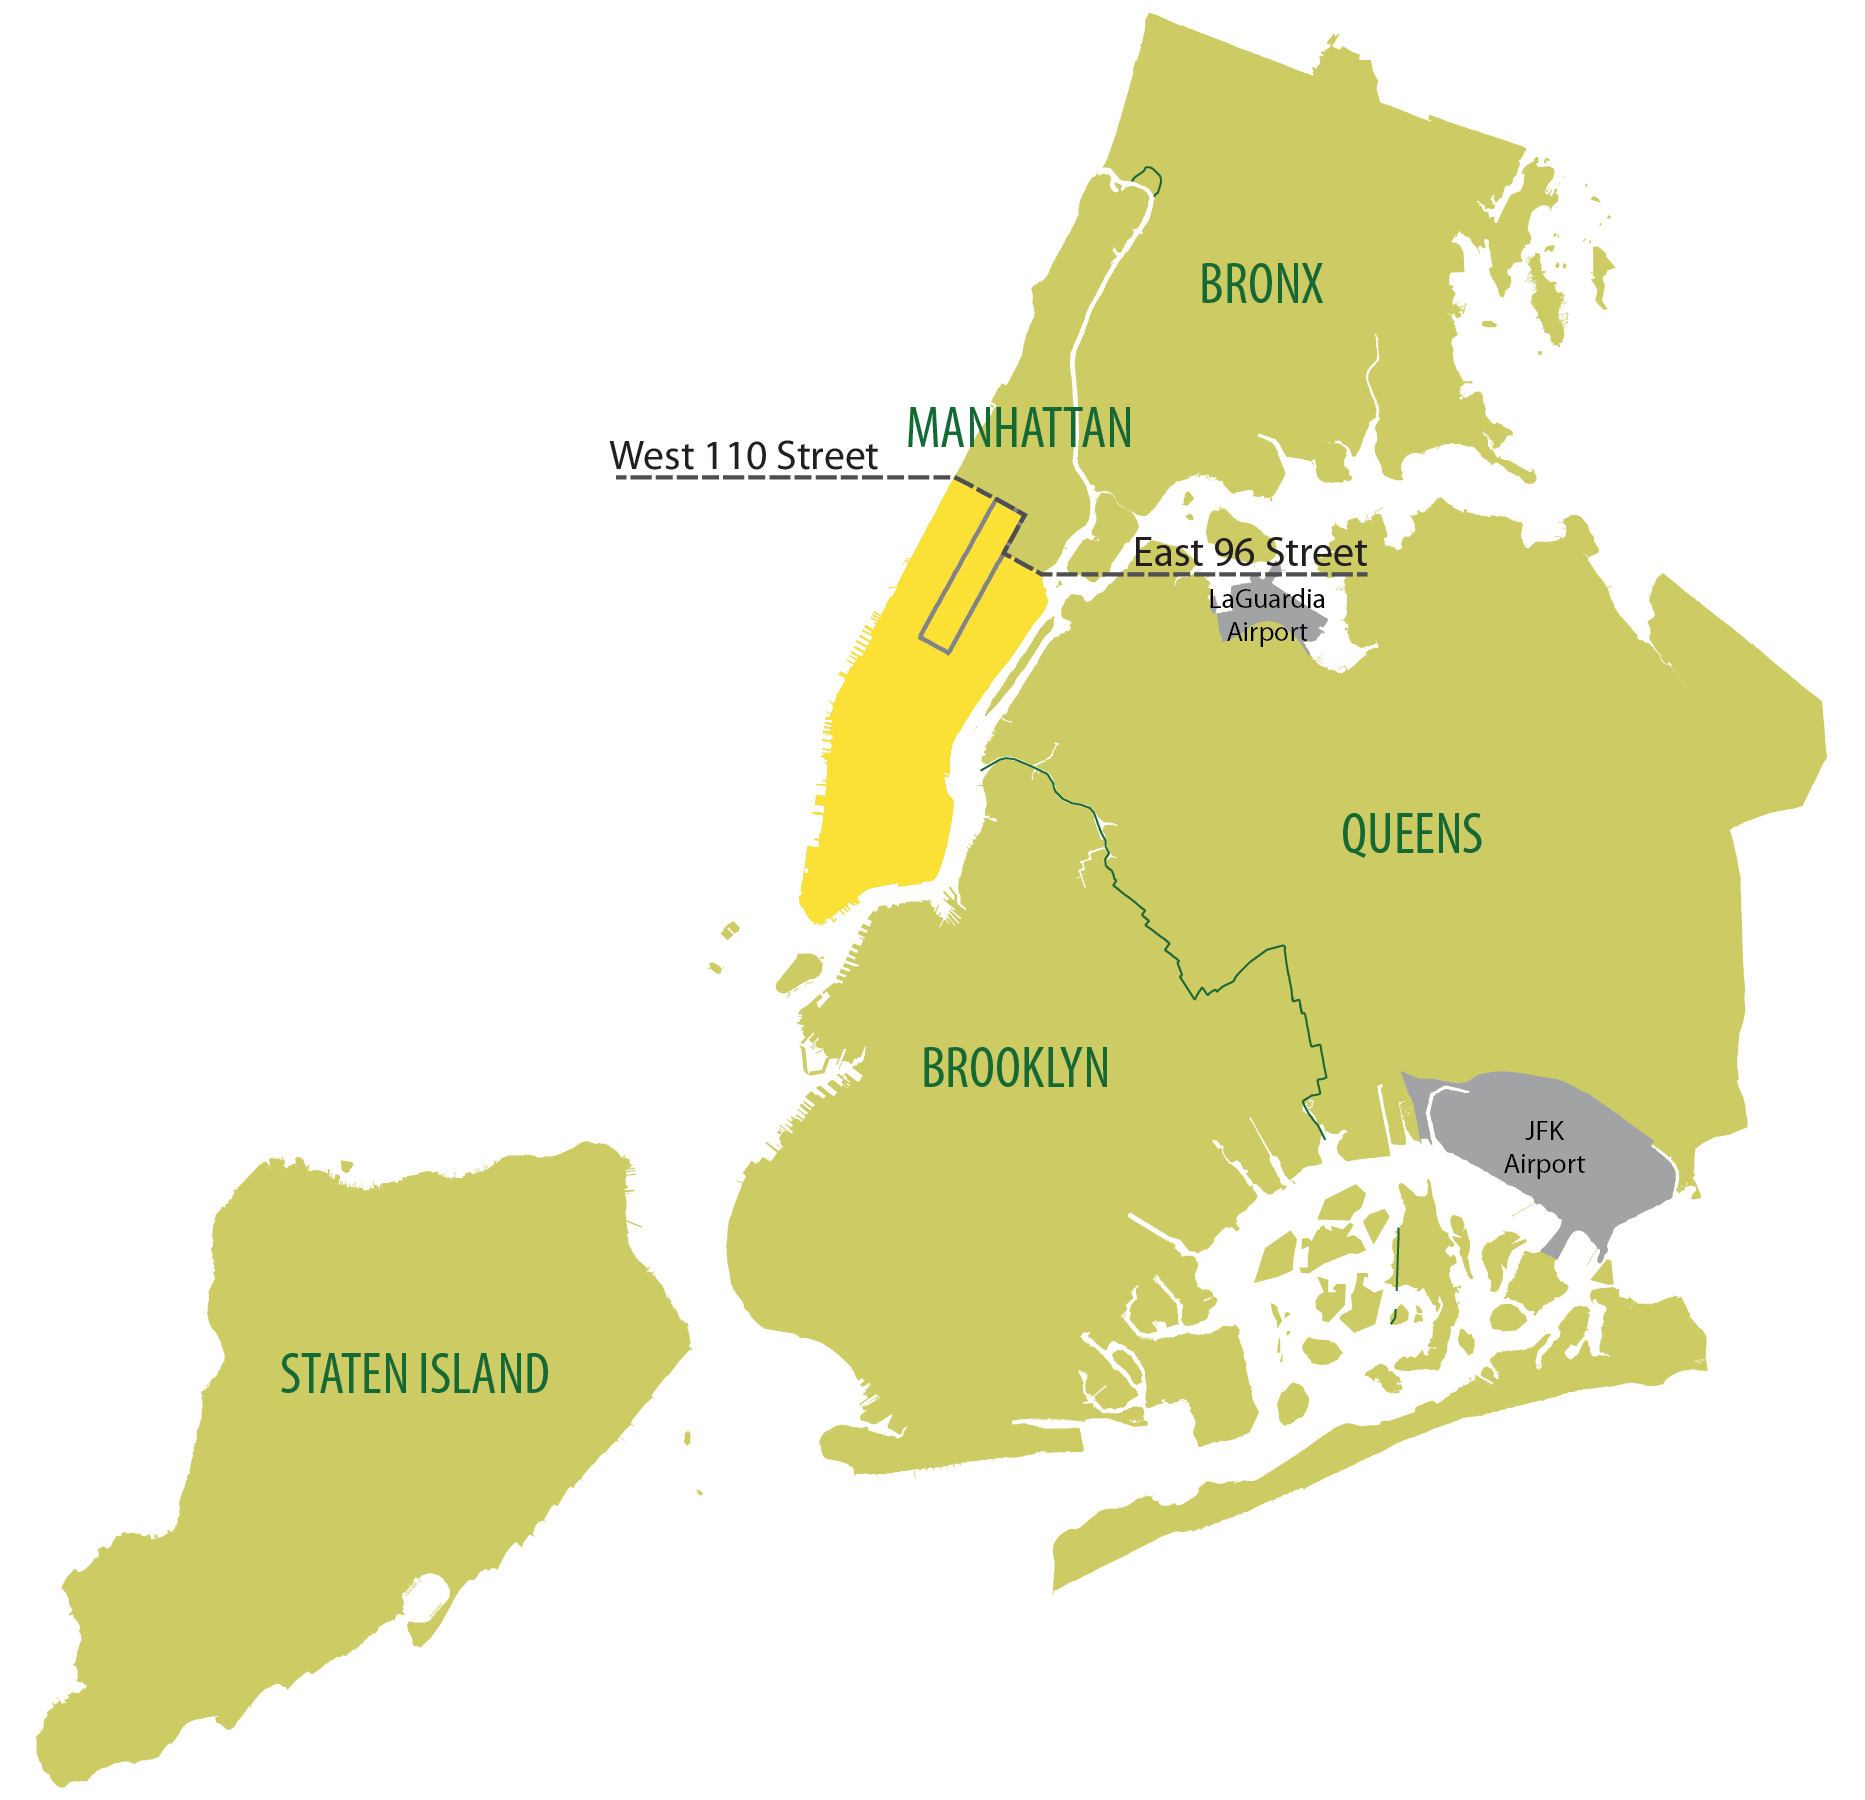
\includegraphics[width=\linewidth]{map_service_area.png}
      \caption{Map of NYC with the green taxi pickup areas colored in green. \cite{boroTaxi}}
      \label{greenZone}
\end{figure}

Figure \ref{greenZone} shows us that the rides for Green taxis are very different than the rides of Yellow taxis.  Yellow taxis for the most part stay around Manhattan, while the Green taxis are all over the city.  This means that, for example, the way the drivers find passengers, the traffic the drivers deal with, the routes that drivers take and the number of stoplights the drivers deal with are different between Yellow taxis and Green taxis.  In addition, the number of trips that Green taxis and Yellow taxis make in a day are very different.  Doing a basic comparison between the 2016 taxi datasets available at NYC Open Data, we see that there are 16.4 million records for Green taxis from January 1, 2016 to June 30, 2016 \cite{green2016} while there are 133 million records for Yellow taxis for the whole year of 2016 \cite{yellow2016}.  

There has been previous work on these datasets which has focused on both the datasets for Yellow and Green taxis; however, given the obvious differences in taxi trip details as well as data size, this report documents my attempt to model trip duration for only the Green taxi data.   In this case, we found that using a basic feed-forward neural net to minmize the root mean squared error (RMSE) of the rounded duration, in minutes, was optimal.  Furthermore, we explore why RMSE was chosen as the loss function instead of the root mean squared log error (RMSLE).  <AND THE ENSEMBLE>


\subsection{Motivation}
Originally, I was going to try to work on the problem of taxi trip duration prediction introduced in a Kaggle challenge \cite{kaggle}.  However, as I explored existing work surrounding this problem, I realized that when most papers look at the NYC taxi data, they either combine Yellow and Green taxi data \cite{blog}, or only focus on Yellow taxis \cite{kaggle}\cite{ucsd}.  Not to mention, most work available has been done by students or through kaggle.

Predicting taxi trip duration is important for multiple reasons.  First, trip duration can be used by a customer to schedule their ride or to estimate the fare for a trip.  Second, it could allow taxi companies to start making, or improve, their ability to chain together rides to increase profit for a driver.  Lastly, having a baseline for what the expected trip duration would allow taxi companies to detect when drivers are taking their passengers on the "scenic route" in order to charge the passengers more.


\section{Related Work}
As I mentioned above, the work on this dataset has been done informally through school projects or Kaggle competitions; however, there is other work related to taxi data.

\subsection{Existing Work on NYC Taxi Trip Duration Prediction}
In July 2017, Kaggle issued a challenge to Kagglers to work on a pre-selected NYC taxi trip dataset in order to predict the trip duration; however, the focus of the competition was to encourage collaboration, so the top publically available kernels are focused on exploring the data in a clear way to benefit the group \cite{kaggle}.  In addition, the few publically available codebases were not from top performers \cite{currie} \cite{yukw} \cite{mk}.  Since it was still a competition to predict the trip duration, Kaggle still provided the means for evaluating the models using RMSLE.  After evaluating this loss function, I decided to go with RMSE as my loss function instead.  I will go into more detail in section \ref{loss}.

Additionally, other students have used this dataset to predict trip duration and made their work publically available; however, none of them used neural nets, which are the new "hot" thing to do because of their ability to fit to a lot of datasets fairly well.  In one paper, they used linear regression and random forests in order to build their model to predict the number of minutes the trip will take and achieved a low RMSE of 5.24 \cite{stanford}.  Another project achieved an RMSE of 4.87 by using a gradient boosting regressor \cite{ucsd}.  I used the second paper that achieved a RMSE of 4.87 as a baseline, which will be discussed in section \ref{baseline}. 

\subsection{Other Work on Taxi Data}
Ferreira et. al. have also used the NYC Taxi data in order to discuss how to best visualize and query datasets such as the NYC taxi data \cite{query}.  While their work is interesting and does use the NYC taxi data, it does not attempt to make any predictions on the trip duration.

It should be noted that in 2015 there was another Kaggle competition to predict the trip duration for taxi data from Porto, Portugal \cite{kagglep}.  One of the top ranking results were published by a group from IBM in which they discuss how they would predict the final destination based on the beginning trip trajectory and would use that to predict the trip duration \cite{ibm}.  However, they were predicting the trip duration based on the initial route of the taxi after picking up a customer, which contains very different data than is available for the NYC taxi data.

\subsection{Other Work on Trip Duration Prediction}
Work has been done to predict when a bus will arrive at its stop using an algorithm based on Kalman Filtering  \cite{india}; however, their work was focused on data collected in India and they needed to be able to analyze the data real time.  First, traffic in India is probably different from traffic in NYC.  Second, bus routes and stops are well defined while taxi routes and start/end locations are not pre-determined until a customer gets into a taxi. 

More work on bus arrival prediction has been done by Biagoni et. al. in which they use a smartphone that is placed on a bus to predict when the bus will arrive at its next stop \cite{et}.  Once again, this is bus data and relies on real time data for a specific route with specific stops.

Additionally, there has been quite a bit of work on predicting travel time on freeways \cite{freewayca} \cite{highway}.  However, driving in a city is very different from driving on a freeway.


\section{Data and Data Challenges}
 

\subsection{NYC Open Data}
New York City made the data for January 2016 - June 2016 of the trip records for the Green taxi data publically available \cite{green2016}. There are approximately 16 million rows.  This data contains the following information:
\begin{itemize}
\item{Vendor ID : One of two vendors}
\item{Pickup and Dropoff Date time: Time and Date when customer was picked up and dropped off}
\item{RateCode ID: Rate (and the code) change based on where the customer is going}
\item{Pickup and Dropoff Location: Contains the lat/long for both of these locations}
\item{Passenger count: Driver recorded number of passengers in the vehicle for the ride}
\item{Information about the fare: Base rate, taxes, tips}
\end{itemize}

I enriched this dataset with two other datasets: weather and sunrise/sunset times.

\subsection{Weather}
Since traffic and taxi use can be heavily influenced by weather, I pulled down some basic stats about the weather for the taxi data being analyzed. The weather for April and March was retrieved from a site run by NOAA \cite{weather}.  There was one record per day containing:
 \begin{itemize}
\item{Minimum/Maximum/Average temperature}
\item{Precipitation: The amount of rain that fell.  Note that a value of T stands for trace}
\item{New Snow: The amount of new snow that fell}
\item{Snow depth: How deep the snow was}
\end{itemize}
Note that both the New Snow and Precipitation columns contained a few values of "T", which stands for trace.  This means that very little snow/rain fell and it was not able to be measured.  Records that had a value of "T" were assigned the value of 0.00001 based on a recommendation in the Journal of Service Climatology \cite{trace}.

\subsection{Sunrise/Sunset}
Lastly, the taxi data was enriched with sunrise and sunset information.  Note that the sunrise and sunset can affect traffic because the sun may get into people's eyes, causing them to slow down.  The sunset and sunrise times were retrieved from a site owned by the US Navy \cite{sun}.


\section{Features Used}


\section {Baseline Model} \label{baseline}


\section{Neural Network}


\subsection{Loss Function} \label{loss}
I debated between using two loss functions, RMSLE and RMSE.  Utlimately, I choose to use RMSE and will explore why in the following paragraph.

Kaggle decided to use RMSLE:

$\epsilon = \sqrt{\frac{1}{n} \sum{(log(p_i + 1) - log(a_i + 1))^2}}$

with a little bit of manipulation of the logs, this transforms into:

$\epsilon = \sqrt{\frac{1}{n} \sum{log(\frac{p_i + 1}{a_i + 1})^2}}$

This shows that, in essence, the model is heavily punished when $p_i < a_i$ as compared to when $p_i > a_i$.  This means that this model will try to avoid predicting under the actual value, but the loss isn't as severe if it goes over.  Thus, minimizing the RMSLE loss is better for finding a model that will predict the minimum trip duration.  Furthermore, because of it's use of the log function, RMSLE would be good for numbers that are going to be large.  For instance, if we were to predict the trip duration in milliseconds or seconds, then RMSLE might be a better choice; however, I choose to focus on predicting the trip duration in minutes, not seconds.

RMSE is calculated as follows:

$\epsilon = \sqrt{\frac{1}{n} \sum{(p_i - a_i)^2}}$

which shows that the model will get equally punished for predicting too large of a value as it will too small of a value.  Thus, I choose to minimize the RMSE when building my model.

\subsection{Neural Network Settings}


\subsection{Testing}

\subsection{Transfer Learning}
Attempt on March Data


\section{Future Work and Ideas}
Combining results from models trained on different loss functions?
Additional features.
Model to predict route.
Geo clustering.




\section{Conclusion}



% conference papers do not normally have an appendix


% use section* for acknowledgment





% trigger a \newpage just before the given reference
% number - used to balance the columns on the last page
% adjust value as needed - may need to be readjusted if
% the document is modified later
%\IEEEtriggeratref{8}
% The "triggered" command can be changed if desired:
%\IEEEtriggercmd{\enlargethispage{-5in}}

% references section

% can use a bibliography generated by BibTeX as a .bbl file
% BibTeX documentation can be easily obtained at:
% http://mirror.ctan.org/biblio/bibtex/contrib/doc/
% The IEEEtran BibTeX style support page is at:
% http://www.michaelshell.org/tex/ieeetran/bibtex/
\bibliographystyle{IEEEtran}
% argument is your BibTeX string definitions and bibliography database(s)
\bibliography{IEEEabrv,taxi}
%
% <OR> manually copy in the resultant .bbl file
% set second argument of \begin to the number of references
% (used to reserve space for the reference number labels box)

%\bibliography{baltimoreBib}
%\bibstyle{filename}
%\nocite{*}
%\begin{thebibliography}{1}
%
%\bibitem{IEEEhowto:kopka}
%H.~Kopka and P.~W. Daly, \emph{A Guide to \LaTeX}, 3rd~ed.\hskip 1em plus
%  0.5em minus 0.4em\relax Harlow, England: Addison-Wesley, 1999.
%
%\end{thebibliography}




% that's all folks
\end{document}

